\documentclass[11pt,a4paper]{article}
% footnote numbering starts with 1 for each page
\usepackage{perpage}
\MakePerPage{footnote}
% No indented footnotes at the bottom of the page
\usepackage[bottom, flushmargin]{footmisc}
\usepackage[greek,american]{babel}
\newcommand{\gr}{\foreignlanguage{greek}}
\usepackage[pdftex]{graphicx}
\title{PROTEUS}
  % \tt = typewriter text
  \author{\tt {\small proteuss@sdf.org}}
  %\date{}
\begin{document}
  \maketitle
\begin{abstract}
\noindent
  Proteus is a decoder and converter for the ancient Greek and Latin
  texts of the TLG and PHI digital libraries.
  The TLG/PHI databases can be searched via a user interface (GUI) and
  complete texts can be extracted and converted to \LaTeX\ source code, pdf
  or plain unicode (utf-8) text for printing or further processing.
\end{abstract}
  \tableofcontents
\section{Introduction}
  The TLG\footnote{Thesaurus Linguae Grecae is a digital library in a CD-ROM
  and it contains all the literary texts written
  in the Greek language from the time of Homer until 1453 A.D.\\
  See: http://www.tlg.uci.edu } digital library contains classical Greek
  texts encoded in a sui generis
  format called {\bf Beta Code}.  This format is very
  efficient\footnote{The Greek texts occupy about
                     600 Mb (uncompressed),
                     and the Latin texts about 80 MB.}
  but it is not  directly readable by word
  processors or text editors.  There are programs\footnote{Diogenes, Musaios,
  Antiquarium, et. al.} that can search the TLG database for words
  or phrases and display chunks of text but cannot display or extract
  complete texts.
  The aforementioned also apply to the Latin corpus
  (PHI CD5)\footnote{
                  PHI5 is a Latin language equivalent of the TLG.
                  It contains virtually all classical Latin literature
                  through to A.D. 200 and some biblical texts in Latin,
                  Greek, Coptic, Hebrew and English. For the list of contents see:\\
                  {\tiny https://web.archive.org/web/20170623105104/http://latin.packhum.org/canon
                    or\\
                  https://web.archive.org/web/20160803141809/http://www.indiana.edu/\textasciitilde letrs/text-tools/textlists/phibibliog.html }
                   }
  and Papyrological/Epigraphical corpus
  (PHI CD7)\footnote{
                       PHI7 has the title: "Greek Documentary" and includes
                       a large collection of documentary papyri
                       and Greek inscriptions. See:\\
                       {\tiny https://web.archive.org/web/20080818140802/http://132.236.125.30/content.html }
                        }
  of the Packard Humanities Institute.
  Proteus can extract complete texts from these corpora
  and translate the Beta Code into Unicode (utf-8)\footnote{utf-8 encoded
  text is compatible with MS Office Word and Open Office Writer.}
  text, or into pdf\footnote{ pdf (Portable Document Format)
  is readable by Adobe Reader, Foxit, kpdf, Evince etc.}
  documents for editing or printing. Optionally it can deliver the \LaTeX\
  source code used to generate the pdf for custom typesetting of the texts.
  It provides a convenient
  interface for searching each corpus canon for an author and for selecting
  particular works from each author for conversion and viewing.
  It can also serve as a useful utility when searching for
  authors since it displays geographical, chronological and genre
  data for each each author/work (when these are available).
  Proteus is not suitable for word searches.  If you need to search the
  TLG/PHI for words or phrases, use
  Diogenes.\footnote{https://d.iogen.es/d/}
  This is by far the best tool for searching or browsing the TLG database,
  and its free. In fact Proteus uses some of Diogenes' programming concepts.
%%%%%%%%%%%%%%%%%%%%%%
% System Requirements
%%%%%%%%%%%%%%%%%%%%%%
\section{System Requirements}
  The conversion from beta code to utf-8 is done by a fast binary
  executable\footnote{The executable called ``{\tt tlg2u}'' and it
  can be used on its own from the command line. See https://github.com/proteusx/tlg2u}
  written in C
  and it controlled via a user interface written in Perl.
  Proteus also needs XeTeX for the automatic typesetting of pdf documents.
  %
  \paragraph{Operating System.}
  Proteus works well with any 64 bit Linux distribution.
  The actual Proteus scripts occupy about 3 Mb of disk space, but if you
  need to install Perl and \TeX{}, you may require up to 350 Mb of disk space.
  In addition, if you transfer the TLG and PHI files from the CD-ROM to
  your hard disk, you will need 800 Mb of additional disk space.
  %
  \paragraph{TLG and PHI CD-ROMs.}
  The TLG and PHI libraries are not included with
  Proteus and you must obtain the CD-ROMs separately. Proteus can
  access the CDs directly, but it will perform better if all the files are
  copied to hard disk directories. The default location for the TLG nad PHI files is
  {\tt /usr/local/CDROMS/} and the expected directory structure is:
  \begin{verbatim}
              /usr/local/CDROMS/
                                |-- phi5
                                |-- phi7
                                |-- tlg
  \end{verbatim}
  Copy the contents of the CDs to the above directories.  If you install the
  files somewhere else you need to edit the top 3 lines the configuration
  file {\tt proteusrc} so that proteus can find them.
  %
  \paragraph{Perl.}
  It requires a Perl interpreter (version 5.8.6 or greater) and the
  modules Perl-Tk, Storable and File-Slurp.
  %
  \paragraph{XeTeX.}
  Proteus uses XeLaTeX\ to automaticaly typeset the texts into pdf documents.
  This is part of the \TeX\ open source typesetting system. \TeX\ is used
  for decades by academics for scholarly publications and can typeset high
  quality documents. A \TeX\ installation is
  required and must include the packages XeTeX, xtab, latexmk and xgreek
  (provides Greek hyphenation and Greek numerals). The package philokalia
  (a very nice antique font with some interesting ligatures and other features)
  is optional.  If XeTeX is not
  installed, the program will function with the pdf option disabled.
  %
  \paragraph{Unicode Polytonic Greek Fonts.}
    Proteus needs unicode fonts in the system for its user interface
    and for the typesetting.
    Can utilize True Type (ttf) or Open Type (otf) fonts for typesetting.
    Fonts are compatible if they include glyphs in the UCS ranges
    0370 - 03FF (Greek) and 1F00 - 1FFF (Greek Extended).
    Examples of such fonts are Palatino Linotype and the latest version\footnote{
                Included with Windows 7/10.
                The Times New Roman fonts as found
                in Windows XP or the open sourced version do not include the
                 polytonic characters.}
    Times New Roman.  The older WinGreek type fonts are not compatible.
    Polytonic unicode fonts can be downloaded freely
    from the Greek Font Society.\footnote{
                https://www.greekfontsociety-gfs.gr/typefaces
                }
    For example, GFS Didot and GFS Neohellenic are excellent typefaces.
%%%%%%%%%%%%%%%%%%%%%%
% Linux Installation
%%%%%%%%%%%%%%%%%%%%%%
\section{Linux Installation}

    \paragraph{Installation of CDROMs.}Copy the TLG and PHI files from the CDs
    to the default directories as indicated in the previous section.
    %
    \paragraph{Download} and unpack the contents of the compressed release
    archive somewhere in your home directory.
    %
    \paragraph{Unicode Fonts.}
      Verify that the system has some unicode fonts installed, as described above.
      If not, download and install fonts as provided by your Linux distribution.
      Some fonts are included in the release and these can be installed in the directory
      {\tt /usr/local/share/fonts} by typing  {\tt sudo make fonts}.
      %
    \paragraph{XeTeX.}
      Next you need to verify that your \TeX\ installation has all the required modules.
      Most Linux distributions offer \TeX\ as an option. If possible, install
      TeX Live\footnote{http://www.tug.org/texlive/acquire.html} with all the
      Greek language options enabled and make certain that XeTeX, xgreek, xtab, latexmk
      and philokalia (optional) packages are installed.
      To test your installation, give the command:~ {\tt make xetex\_test}.~~
      If everything is in order your default pdf reader will open displaying
      some readable Greek text.  If the command gives errors and no pdf is produced
      look at the log file {\tt \~{}test.log}  and check your
      \TeX\ installation. You many need to update XeteX and Fontspec.
    %
    \paragraph{Perl.}
      All Linux distributions have Perl installed by default.  Make certain that
      the required modules are installed. If not, do whatever is required
      by your distribution to download and install the missing modules.
      Alternatively you can test and install any missing modules with the
      command:\\*  {\tt \hspace*{2cm} sudo make perl\_test}
    %
      \paragraph{Installing Proteus.}
      Installation is done through the makefile:\\*
      {\tt \hspace*{2cm} sudo make install}.\newline
      This will install everything in the directory {\tt /usr/local/proteus}.
      If you wish to install somewhere else, edit the {\tt INSTAL\_PREFIX}
      variable in the makefile .
      Thereafter you can start Proteus from the icon in the start menu
      (usually found in the category ``Office'') or by typing:~ {\tt proteus}
      in a terminal.
    %
    %
    \paragraph{Directories.}When running Proteus for the first time, a hidden directory {\tt .proteus}
      will be created in your home directory to keep your personal defaults and output files.
      Also, you may be requested to point to the directories where the TLG/PHI
      files are located. These locations will be stored and thereafter
      Proteus will not ask again unless there is a change.
      These locations can be altered from ``Files'', ``Corpus Directories''.
      The default location for output files (pdf, utf, etc.) is the
      subdirectory {\tt \~{}/.proteus/books}.  You can later change this
      to wherever you like, via the menubar ``Files", ``Output Directory".
    %
    \paragraph{Uninstalling.}
      To completely clear Proteus from your system give the command:~
      {\tt sudo make uninstall}.  This however will not
      delete the directory {\tt \~{}/.proteus}
    %%%%%%%%%%%%%%%%%%%%%%
    % Windows Installation
    %%%%%%%%%%%%%%%%%%%%%%
  %\subsection{Windows}
  %  If you happen to have the DVD that includes Proteus, Diogenes
  %  and the\newline TLG/PHI data all you need to do is
  %  run\footnote{Windows 7 and Vista
  %                must run the installer
  %                as ``administrator''}
  %  the installer ``Proteus-setup.exe'' and everything required will be installed
  %  automatically. Otherwise unzip the contents of compressed archive somewhere
  %  in your hard drive and run the installer. It will install Proteus,
  %  TeXLive (scaled down version) with all the required  packages and
  %  modules as well as some required fonts.
  %%
  %  % \newpage
  %  \paragraph{Directories.}When the installation is finished, double click
  %    on the desktop shortcut and when
  %    requested point to the directories where the TLG/PHI files are located.
  %    These will be stored and thereafter Proteus will not ask again
  %    unless there is a change.
  %    These locations can be altered from ``Files'', ``Corpus Directories''.
  %    The default location for the output files (the created pdf and utf documents)
  %    is the subdirectory \verb+C:\Program Files\Proteus\books+.
  %    You can later change this to wherever you
  %    like via the menubar ``Files", ``Output Directory".
    %%%%%%%%%%%%%%%%%%%%%%
    %       Usage
    %%%%%%%%%%%%%%%%%%%%%%
  \newpage
\section{Using Proteus}
  \subsection{Searching}
    \subsubsection*{Authors List.}When Proteus starts, it presents  a
                list of all the authors in the selected corpus.

          \begin{figure}[htp]
            \begin{center}
              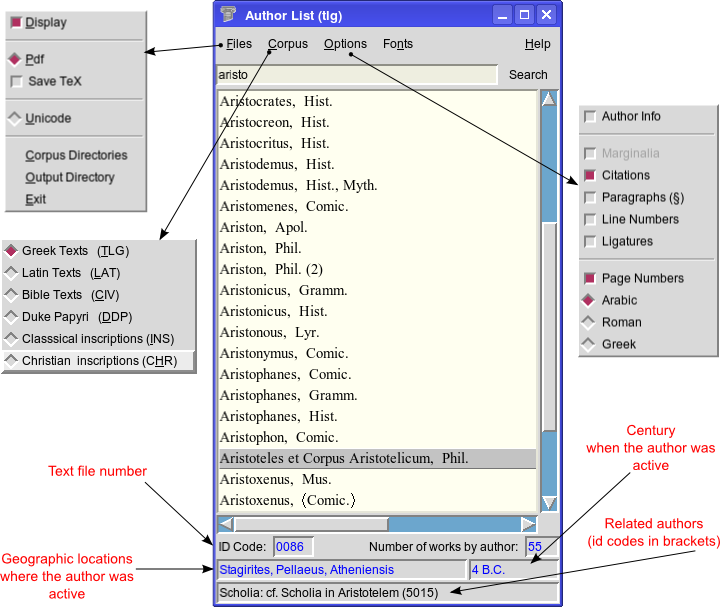
\includegraphics[scale=0.6]{../images/authors-en.png}
              \caption{ {\small
                          The authors window displaying
                            the TLG corpus (over 3500 authors).
                            The expanded menus are also shown.
                            The window decorations depend
                            on the platform. QtCurve on Linux
                            is shown here.
                        }
                      }
            \end{center}
          \end{figure}

      You can locate any author by typing a few letters in
      the search box above the list. This causes the list to display only authors
      whose name includes the given letter combination. For example, typing
      \verb| herod | the list will only display: Herodianus, Herodas, Herodotus, ... etc.
      The list can be searched by epithet or genre, for example;
      typing \verb| lexic | will display all the lexica in the database, or typing
      \verb| hist | will retrieve all the historians.
      You can also search using Regular Expressions. For example typing the sequence
      \verb| ^h.*tus | will yield: Heraclitus and Herodotus.
    %
\newpage
    \subsubsection*{List of Works.} Selecting\footnote{Selection can be done
        with mouse clicking or cursor up/down arrows. Faster movements are possible
        with Page Up/Down or using the side bars.} any author from the list will
        open a second list showing all the works, by the selected
        author.

              \begin{figure}[htb]
                \begin{center}
                  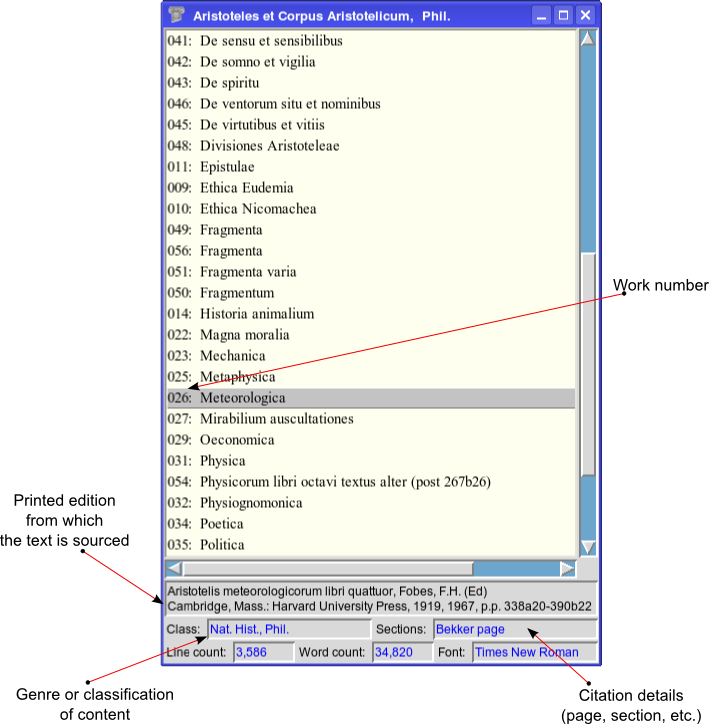
\includegraphics[scale=0.6]{../images/works-en.png}
                  \caption{The works window.}
                \end{center}
              \end{figure}

  %
  \subsection{Unicode text output}From the menu bar select ``Files"
    and click the option ``Unicode". All options not pertinent to unicode
    text conversion will be disabled.
    Now double click\footnote{or select and press ``Enter".} on one of the works.
    This will extract the text, encode it in utf-8 and save it in a file.
    A pop-up window will ask for a file name. You may accept the default or rename
    it, but it is wise to keep the postfix ``.utf".
    This file will be passed on to the default word processor for display.
    The word processor may ask about the encoding of the file.  Select
    ``Unicode(utf-8)". Also select the default font.\footnote{LibreOffice Writer only.}
    Finally, within the word processor, select all the text (CTRL-A) and put
    it in a polytonic Greek font.  If you have selected options that display marginalia,
    citations, paragraphs  numbers or line numbers in the margins it is advised that you
    select a {\bf monospaced font} such as Consolas or Courier.
    This is to keep the line width constant so that the margins will have a uniform
    appearance.
              \begin{figure}[htb]
                \begin{center}
                                        %% scale=l b r t
                  \fbox{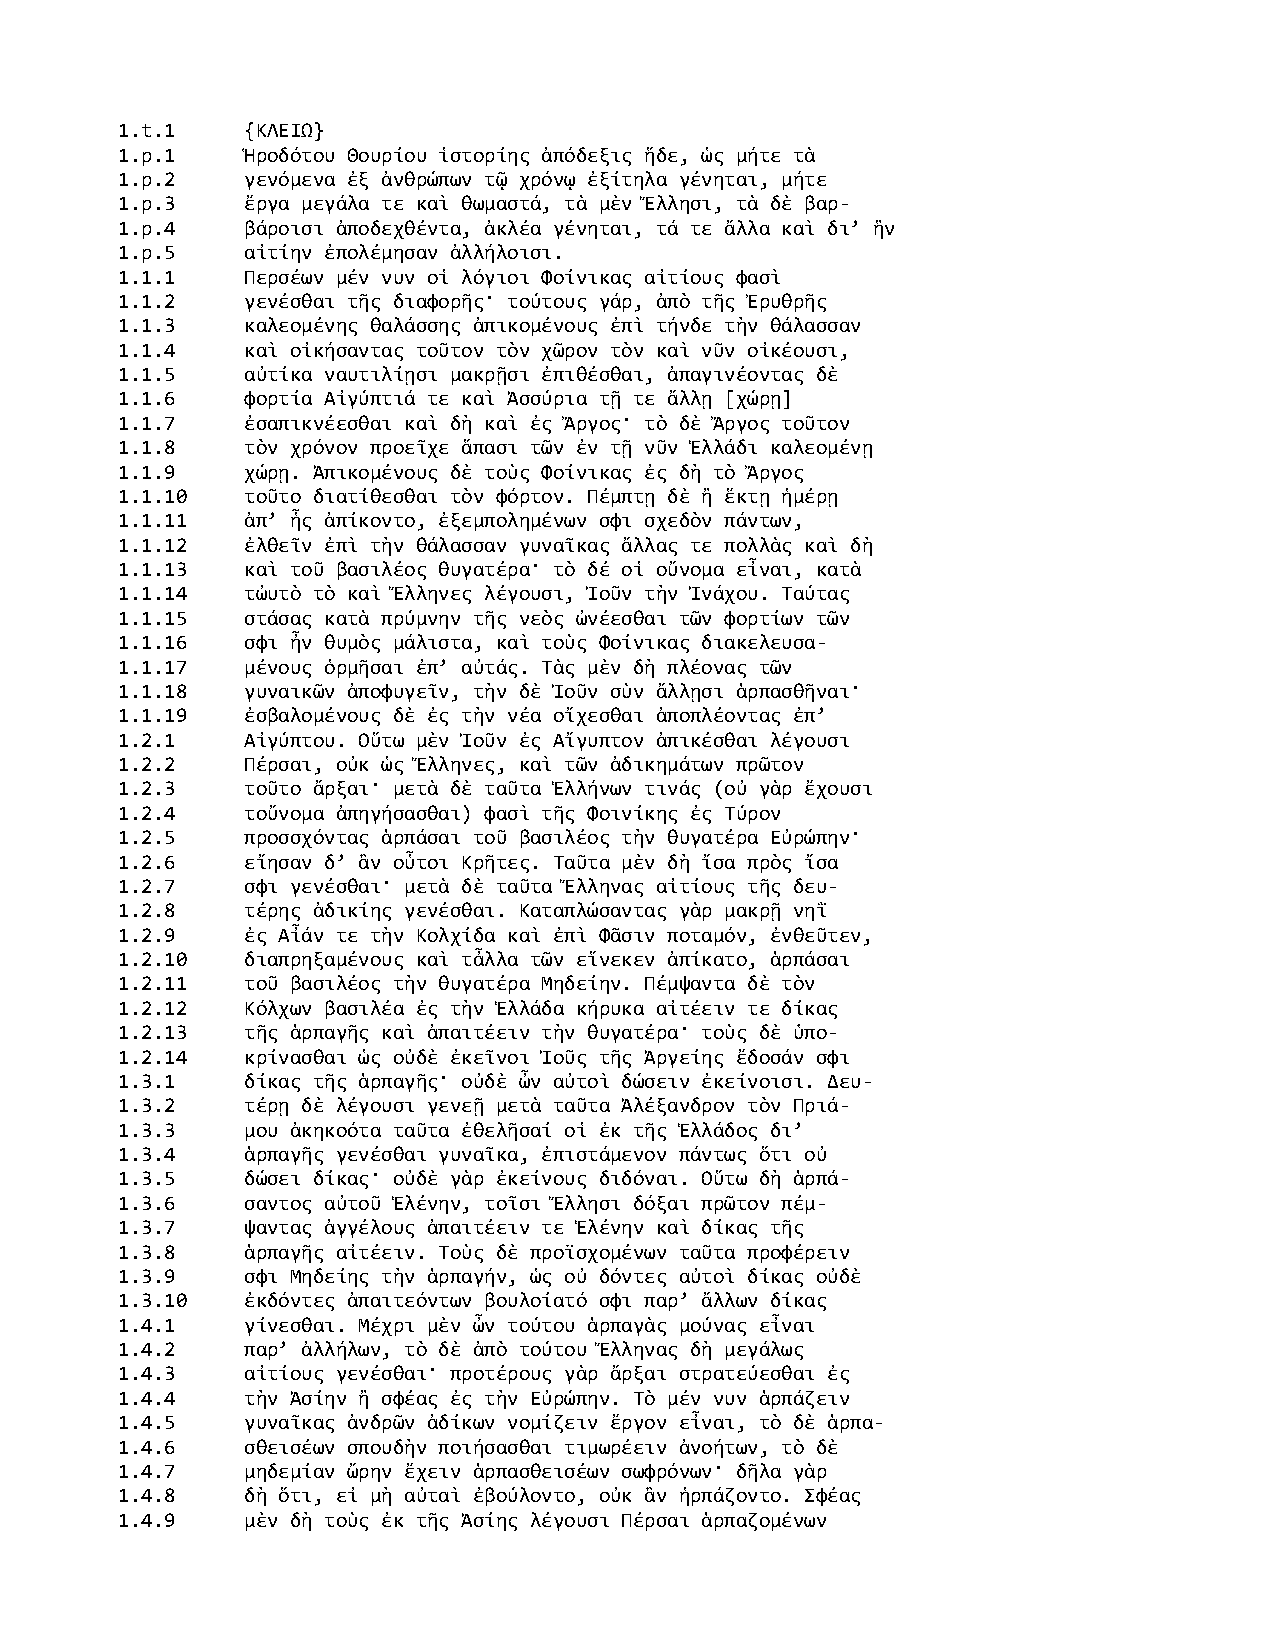
\includegraphics[scale=0.7,trim = 1cm 16cm 5cm 1cm, clip]{../images/herod1.pdf}}
                    \caption{Example of utf-8 text (citations option enabled)
                           displayed with MS Word in 12pt monospaced Consolas font.
                           The citation numbers are shown on the left margin.
                           Title lines are denoted by ``t'' and enclosed in
                           brackets (\{\}).
                           Proems are denoted by ``p''.
                           Note the use of the monospace font to keep
                           margins aligned.}
                \end{center}
              \end{figure}
  %
  \newpage
  \subsection{Pdf document output}From the menu bar select ``Files" and click the
    option ``Pdf". All options pertinent to unicode text conversion will be
    enabled. Selecting and double clicking a title in the author's works
    list will generate a pdf file and pass it to the pdf viewer.  Pdf output
    produces formated text and has several typesetting options to
    choose from.\footnote{Document conversion may take some time depending
    on the number of works of the author and the size of the work selected
    for conversion.  Some author files may be very large.
    For example St. John Chrysostom's file contains 402 works, or Stobaeus anthology
    is 1260 pages long. So be patient.}
              \begin{figure}[htb]
                \begin{center}
                  \fbox{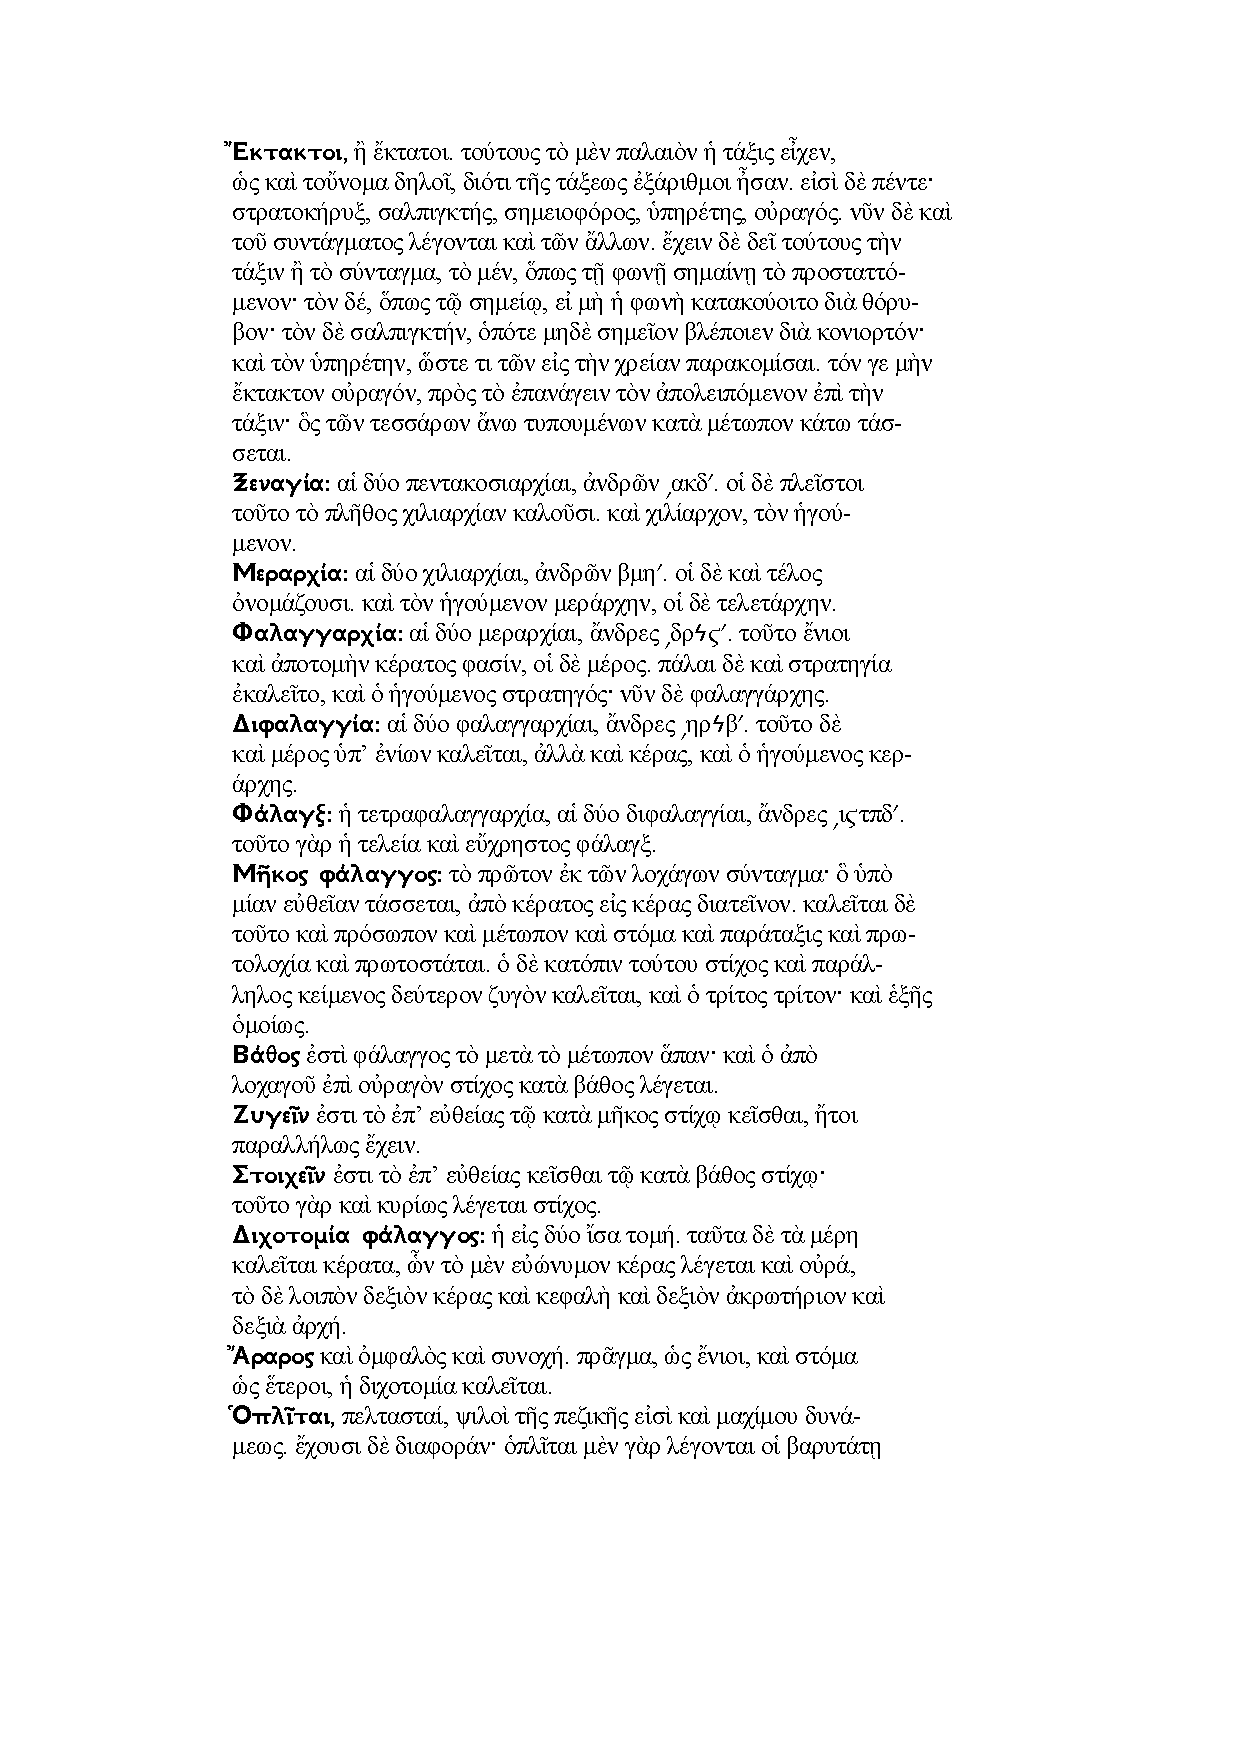
\includegraphics[scale=0.7,trim = 2cm 152mm 4cm 2cm, clip]{../images/onom-2.pdf}}
                  \caption{Example of automatic pdf output.
                           Suda's Onomastikon typeset in Times New Roman.
                           Note that the lemata are accentuated
                           in GFS Neohellenic Bold.  Such font combinations
                           are possible with the Font Selector.
                           }
                \end{center}
              \end{figure}
  %
  %%%%%%%%%%%%%%%%%%%%%
  %   Corpus Selector
  %%%%%%%%%%%%%%%%%%%%%
  \subsection{Files menu}
    \begin{itemize}
      %
      \item {\bf Display:} Display the output file immediately by sending
      it to word processor or
      pdf Reader. Regardless of this option the file
      will be written to  the output directory for later use.
      %
      \item{\bf Pdf:} Save the output as a pdf file.
      %
      \item{\bf Unicode:} Save the output as utf-8 encoded text file.  This file may be
        imported by Word, Open Office or whatever.
      %
      \item {\bf Save TeX:} Save the \TeX\ source file (as \verb|file_name.tex|).
      This file contains the unicode text and all the typesetting instructions.
      Advanced users may wish to edit this file to alter the automatically
      produced pdf document. This file can be compiled manually like so:
      \begin{center} {\tt xelatex file\_name.tex}\end{center}
      %
    \end{itemize}
  \subsection{Corpus selector}
    The item labeled ``Corpus'' presents a menu to select one
    of the following corpora:
    \begin{itemize}
      \item Greek texts (TLG).
      \item Latin texts (LAT).
      \item Bible texts (CIV).
            Greek, Latin and English Bible texts.\footnote{
                      PHI5 also includes a Coptic
                      and a Hebrew Bible but
                      Proteus cannot convert these. I do not have the specifications
                      for Hebrew or Coptic beta code.                        }
      \item Duke Documentary Papyri (DDP).
      \item Classical Inscriptions (INS).
      \item Cristian  Inscriptions (CHR).
    \end{itemize}
    The 3 bracketed letters are the filename prefix of each corpus. For example the Greek
    texts have filenames are of the form tlgxxxx.txt and the bible texts civxxxx.txt,
    where xxxx is the four digit id number of the author.
    The LAT and CIV files are part of PHI CD5
    and the DDP, INS and CHR are part of PHI CD7.
  %%%%%%%%%%%%%%%%%%%%%
  %      Options
  %%%%%%%%%%%%%%%%%%%%%
  \subsection{Options menu}
    This is a brief description of the available options.
    Some items are only pertinent to pdf only and are disabled when the utf option
    is selected.\footnote{Clicking on the
    perforated line on the top of a menu will cause the menu to
    tear off from the menubar and stay open.}
    \begin{itemize}
    %
    \item {\bf Author Info:} Details of the printed edition from which the text
         is sourced, geographical and chronological details of the author are
         printed at the header of the pdf (or at the bottom of the utf) file.
    \item {\bf Marginalia:} Some texts contain marginal notes. Selecting this option will
    print these notes on the right margin. The program automatically detects
    the existence of marginal notes. If the text has no marginalia the option
    will be deactivated (greyed out).
    %
    \item {\bf Citations:} All texts have numbered entries for book, chapter, section, etc.,
    These vary from text to text and the definitions of the numbers appear at the bottom
    right hand corner of the works window. This option will display all these numbers
    in the left margin.
    %
    \item {\bf \S\ :} Show section numbers in the left margin. Not all texts
    have section numbers. If the text has section numbers this is shown at the
    bottom right hand corner of the author's work list.
    %
    \item {\bf Line Numbers:} Print the line numbers (every fifth line) on the right margin.
    %
    \item {\bf Ligatures:} Enable ligatures for fonts that have them.  These are
    available with only a few fonts. To see its effect use the font Philokalia
    and check this option.
    \begin{figure}[htb]
      \begin{center}
        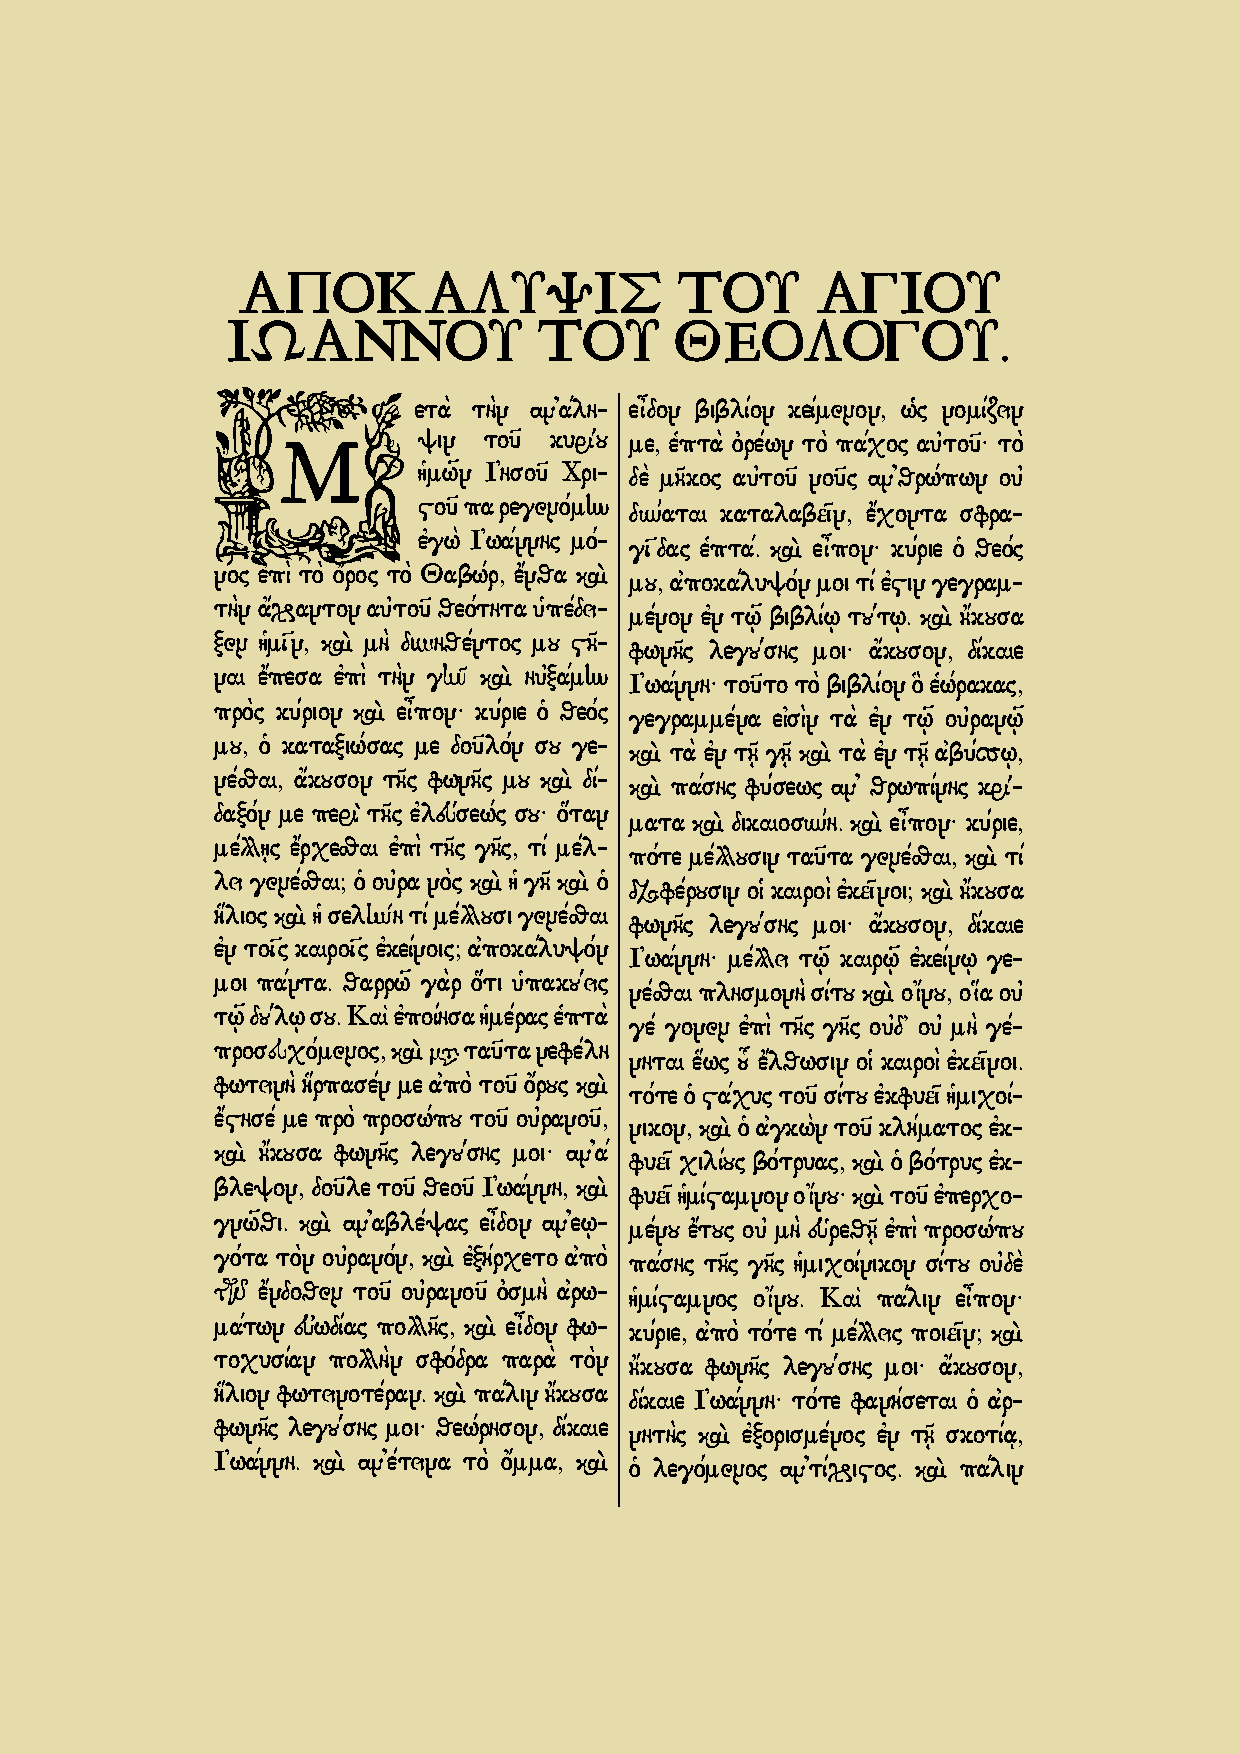
\includegraphics[scale=0.7,trim = 2cm 15cm 2cm 2cm, clip]{../images/apok.pdf}
        \caption{This text is typeset with the Philokalia font
                 with Ligatures enabled.  The TeX source code
                 was saved and its preamble was customized to
                 format the text in two columns set in a coloured
                 backround.}
      \end{center}
    \end{figure}
    %
    \item {\bf Page Numbers:}  Checking this option will show the page numbers at
    the bottom margin.  There is a choice of Arabic, Roman or Greek numerals.
    %
    \end{itemize}
  %%%%%%%%%%%%%%%%%%%%%%
  %       Fonts
  %%%%%%%%%%%%%%%%%%%%%%
  \subsection{Fonts selector}
    The ``Fonts" button, on the menu bar, opens the font selection panel.
    Although the whole text may be typeset with one font (e.g. Times New Roman or Cardo),
    a more professional appearance can be achieved with the use of the options below.
    \paragraph{System fonts.} These are the fonts installed in the operating system.
      Any of these can be used provided that it has the required glyphs.
    \begin{figure}[htb]
      \begin{center}
        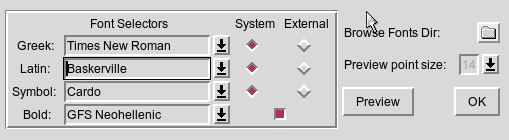
\includegraphics[scale=0.6]{../images/font-selector.png}
        \caption{The Font Selector window}
      \end{center}
    \end{figure}
    \paragraph{External Fonts.} Proteus can also use fonts that are not installed and these
    are called External fonts\footnote{External fonts are specified by their font
      filename whereas installed fonts are specified by their font family name.
    For example the font file times.ttf when installed provides the font family ``Times New Roman'' }. Such fonts are .ttf or .otf files residing
    somewhere other than the system's font directory.\footnote{
                          The default location for such fonts is
                        {\tt /usr/local/proteus/fonts}}
    You can browse for external fonts by clicking the button ``Browse Fonts Dir".
    The four drop down selection lists enable the independent selection of fonts for
    Greek, Latin,symbols and for bold Greek text.
    \paragraph{Greek Font.}This font is used for the Greek text. Use the preview panel
     to verify that the selected font possesses all the characters (glyphs) needed
     for the Greek script.
    \paragraph{Latin Font.}This font is used for Latin text.
      Frequently Latin text
      is found embeded in the Greek text.  Some fonts have very good
      Greek but poor (or not at all) Latin script (or vice-versa)
      hence we may wish to mix Greek and Latin characters from different fonts.
    \paragraph{Symbols Font.}Some fonts may not possess a complete selection
      of special symbols such as Stigma(\gr{\stigma}),
      Koppa(\gr{\qoppa}), Sampi(\gr{\sampi}), daggers(\dag, \ddag)
      etc.,\footnote{Examples of symbol rich fonts are
                     Cardo and Times New Roman (the latest version).}
      and we may wish to use the symbols from a symbol rich font,
      without using it for the rest of the text.
    \paragraph{Bold Font}There are cases, such as in lexica, where a more aesthetic
      effect is achieved if the bold face of a different font is used. We have
      found for example that the bold face of GFS Neohellenic looks good with
      Times New Roman or GFS Didot. For example see Figure 4.  This feature is
      enabled by the check button next to the drop down font list. If this feature is
      disabled the system will automatically use the bold face of each font selected for
      Greek or Latin.

    \paragraph{Preview panel}Clicking ``Preview" will open a panel displaying
      a few lines of sample
    \begin{figure}[htb]
      \begin{center}
        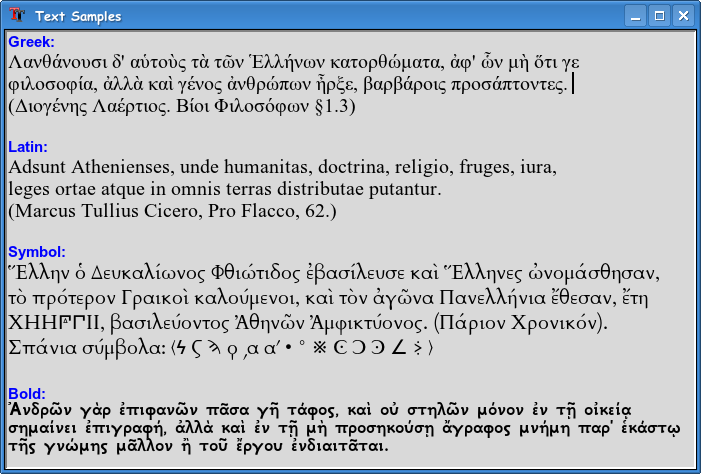
\includegraphics[scale=0.6]{../images/textsamples.png}
        \caption{The Font Preview window}
      \end{center}
    \end{figure}
      text for each selected font.\footnote{Preview is only possible with system fonts.}
      In this way we can inspect the fonts before use. The size of the font in the
      preview can be adjusted with the ``Preview point size" option.
  %%%%%%%%%%%%%%%%%%%%%%
  %     Filenames
  %%%%%%%%%%%%%%%%%%%%%%
  \subsection{Output file names} The TLG CD-ROM, for example,
    has one file for each author. For
    example all works by Homer are stored in the file {\tt tlg0012.txt}. Within
    this file, work no.\ 1 is the Iliad and work no.\ 2 is the Odyssey.
    If we extract the Iliad, the
    default filenames will be: {\tt tlg0012\_001.utf} for the unicode file and
    {\tt tlg0012\_001.pdf} for the pdf file. The tlg file number is shown at the
    bottom of the authors list
    and the work number is shown in the works list on the
    left of each work title.
    This convention also applies to the other corpora each of
    which has its own distinctive prefix. (lat, civ, ddp, ins and chr).
\section{Acknowledgments}
    This project was conceived after reading Peter Hesling's
    notes on Beta Code and Diogenes. {\tt https://d.iogen.es/d/}\\*[2mm]
    The beta code to unicode conversion routine writen in C
    was inspired after reading the utility {\tt tlgu} by Dimitri Marinakis.
    {\tt http://tlgu.carmen.gr/}
\end{document}
